\chapter{Tinjauan Pustaka}

\section{Satelit LAPAN-A3}

\begin{figure}[!ht]
\setlength\belowcaptionskip{-0.7\baselineskip}
\begin{center}
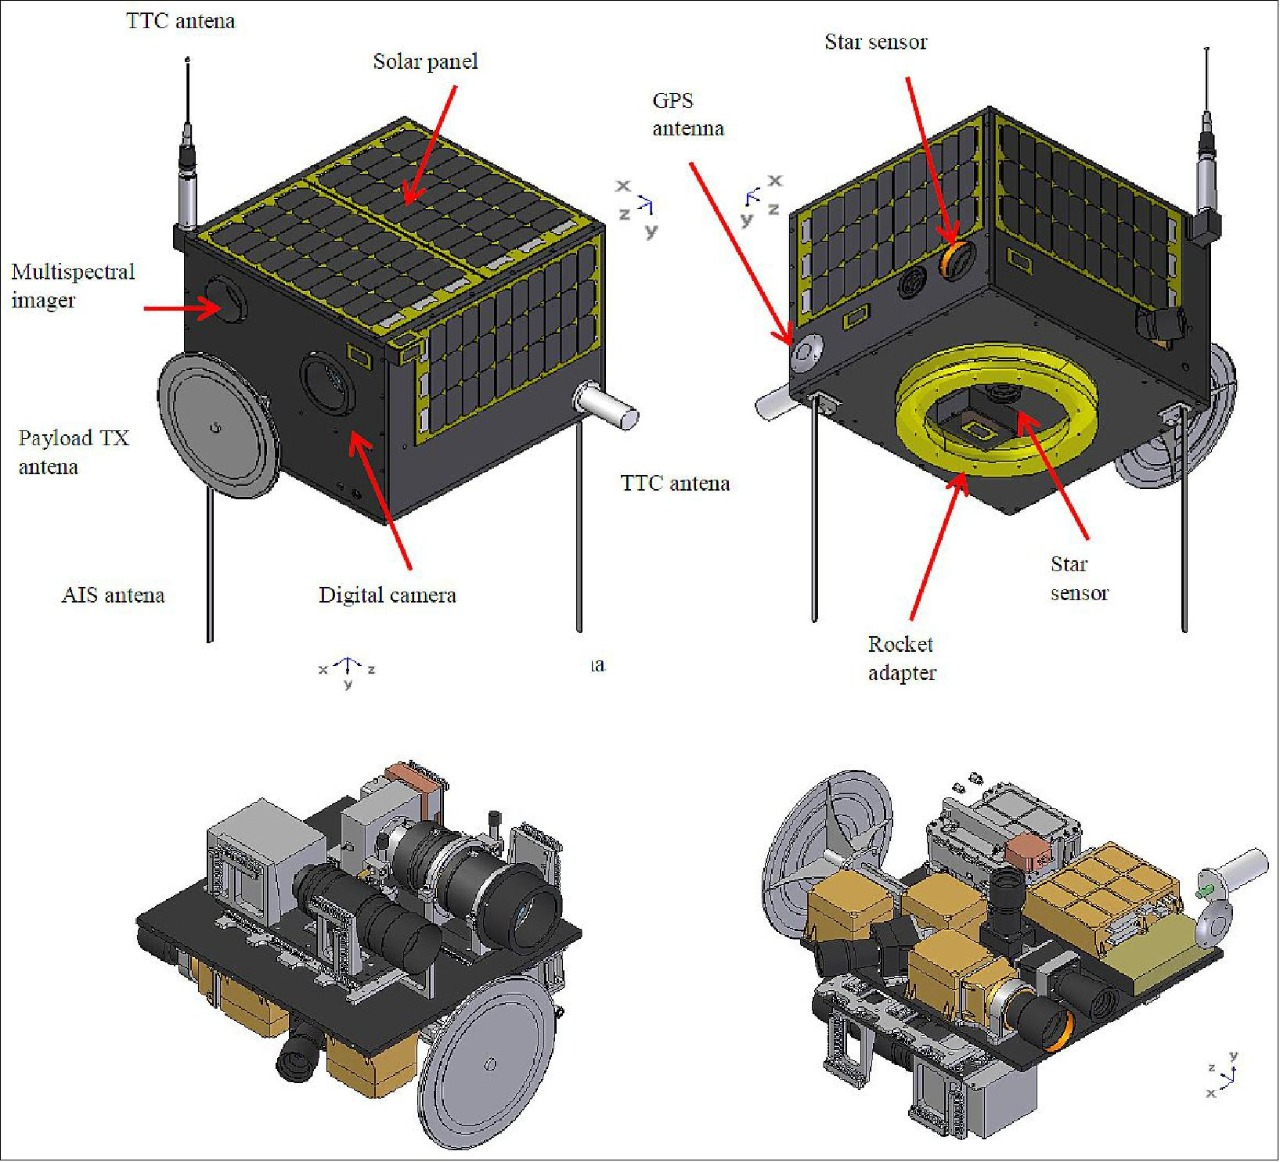
\includegraphics[width=0.7\textwidth]{fig/a3overview.jpg}
\caption{Konfigurasi LAPAN-A3}
\label{fig:a3overview}
\end{center}
\end{figure}

\section{Persamaan Termal Multi-nodal Satelit}

\section{Machine Learning}

\subsection{Koefisien Determinasi (R2)}

\subsection{Root Mean Square Error (RMSE)}

\section{Perangkat Lunak}

\subsection{Python}

Python adalah bahasa pemrograman umum yang diciptakan oleh Guido van
Rossum. Python umum digunakan untuk menyelesaikan permasalahan sains
data \cite{boschetti2015}. Bahasa ini dipilih untuk melakukan perhitungan dan
pemodelan dalam karya tulis ini karena memiliki modul pemrograman yang
cukup lengkap, tidak terikat biaya lisensi, dan kode sumber-nya dapat
diakses secara publik. Versi bahasa Python yang digunakan pada karya
tulis ini adalah 3.10.

\subsection{Pandas}

Pandas adalah modul pemrogaman untuk bahasa Python yang diciptakan oleh Wes
McKinney. Modul ini biasa digunakan untuk mengolah dan menganalisis objek data
seperti baris dan kolom tabel \cite{reback2022}. Pada karya tulis ini, modul Pandas
digunakan untuk mengolah sumber data mentah berupa data telemetri satelit LAPAN
A3 agar dapat diproses lebih lanjut pada tahap pembuatan model termal satelit.

\subsection{Numpy}

Numpy adalah sebuah modul Python yang diciptakan oleh Travis Oliphant. Modul
ini digunakan untuk melakukan operasi pada matriks multi-dimensional secara
cepat dan efisien \cite{harris2020}. Karya tulis ini menggunakan Numpy untuk
menghitung dan menyimpan variabel-variabel yang dibutuhkan model termal satelit
seperti matriks sudut Euler satelit, matriks posisi satelit, dan lain-lain. 

\subsection{Matplotlib}

Matplotlib adalah modul Python untuk membuat plot dan grafik 2D \cite{hunter2007}.
Modul ini diciptakan oleh John Hunter dan umum digunakan pada proyek sains data
sebagai sarana visualisasi data. Karya tulis ini menggunakan modul Matplotlib
untuk menggambarkan hasil pemodelan termal satelit.

\subsection{Scikit-learn}

Scikit-learn merupakan modul pengolahan data, pembuatan model, validasi, dan
pengukuran performa model Machine Learning dalam bahasa Python \cite{pedregosa2011}.
Modul ini pertama kali dikembangkan oleh David Cournapeau pada 2007 dan
mencakup algoritma-algoritma Machine Learning untuk skala menengah.
Scikit-learn digunakan untuk pembuatan model Machine Learning pada karya tulis
ini.

\subsection{Skyfield}

Skyfield adalah sebuah modul astronomi untuk perhitungan posisi bintang,
planet, dan satelit yang mengorbit di sekitar Bumi [@rhodes2019]. Modul ini
ditulis oleh Brandon Rhodes dan menggunakan implementasi algoritma SGP4 dalam
bahasa Python \cite{rodriguez} untuk memprediksi dinamika orbit satelit mengacu
format Two-Line Element (TLE). Karya tulis ini menggunakan Skyfield untuk
mensimulasikan orbit LAPAN A3 selama periode observasi.

